\documentclass[a4paper,oneside,12pt]{book}
\usepackage{BUPTthesisbachelor}
\usepackage{setspace}

\usepackage[final]{pdfpages}

\usepackage{listings}
\usepackage{xcolor}

\usepackage{amssymb}
\usepackage{bm}

\usepackage{algorithm}  
\usepackage{algorithmicx}  
\usepackage{algpseudocode}  

\lstdefinestyle{sharpc}{language=[Sharp]C, frame=lrtb, rulecolor=\color{blue!80!black}}


%%%%%%%%%%%%%%%%%%%%%%%%% Begin Documents %%%%%%%%%%%%%%%%%%%%%%%%%%
\begin{document}

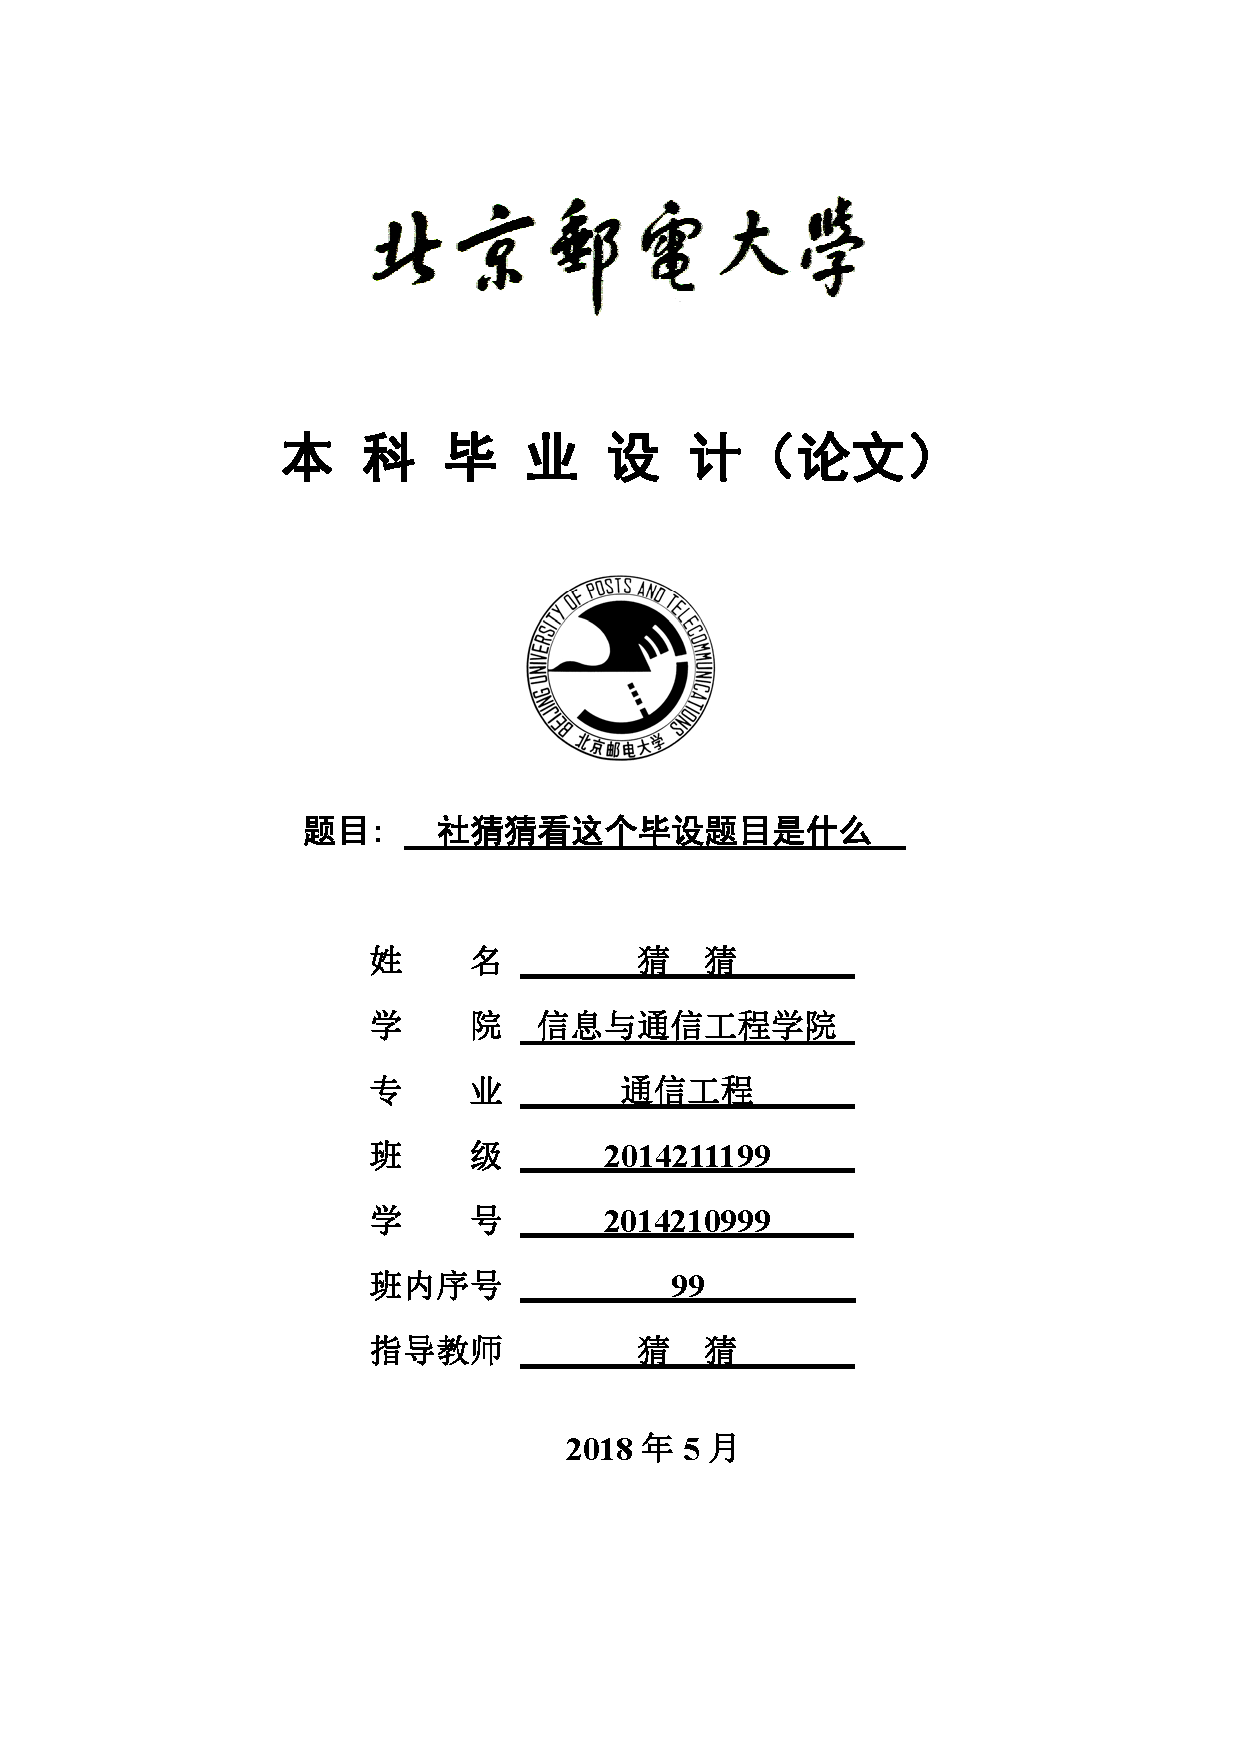
\includepdf{docs/cover.pdf}  
\newpage


\includepdf{docs/statement.pdf} 
\newpage

%%%%%%%%%%%%%%%%%%%%%%%%%%%%%%%%%%%%%%%%%%%%%%%%%%%%%%%%%%%%%%%%%%%%
%                                                                  %
%   Copyright (c) 2010 - 2011 Caspar Zhang <casparant@gmail.com>   %
%                                                                  %
%   This copyrighted material is made available to anyone wishing  %
%   to use, modify, copy, or redistribute it subject to the terms  %
%   and conditions of the GNU General Public License version 2.    %
%                                                                  %
%   This program is distributed in the hope that it will be        %
%   useful, but WITHOUT ANY WARRANTY; without even the implied     %
%   warranty of MERCHANTABILITY or FITNESS FOR A PARTICULAR        %
%   PURPOSE. See the GNU General Public License for more details.  %
%                                                                  %
%   You should have received a copy of the GNU General Public      %
%   License along with this program; if not, write to the Free     %
%   Software Foundation, Inc., 51 Franklin Street, Fifth Floor,    %
%   Boston, MA 02110-1301, USA.                                    %
%                                                                  %
%%%%%%%%%%%%%%%%%%%%%%%%%%%%%%%%%%%%%%%%%%%%%%%%%%%%%%%%%%%%%%%%%%%%

% 你只需要修改下面几行就可以完成大部分内容的填写,
% 这要求你具有一定的LaTeX基础,但是如果你足够聪明,
% 不具有LaTeX基础也可以完成。

% 论文中文题目
\def\thesistitle{社猜猜看这个毕设题目是什么}

% 论文英文题目
\def\thesistitleen{Have a try to guess what the title is}

% Thank Words
\def\thankwords{

此处请写致谢的内容。
它可以有多段。
}
    % Main items 
% Abstract
\clearpage
\thispagestyle{plain}
\phantomsection
\addcontentsline{toc}{chapter}{Abstract}

\centerline{\zihao{3}\bfseries Abstract}

\linespread{1.4}\zihao{-4}
\bigskip

This thesis explores the relationship between focus structure and pronoun resolution among non-native speakers of English and French. Firstly we reviewed the existing literature on the mechanism of focus effect and pronoun resolution. Then through a self-paced reading test, we find that focus, in the form of cleft structure does not necessarily increase the salience of a informational unit, thus may not in some cases make it a preferred antecedent for pronoun resolution. This result is line with previous researches on this topic. In our experiment, We also find that focused subject in French and focused object in English are processed faster, but focused subjects in both languages leads to longer response time of anaphora. Furthermore, our research also shows that the congruence between anaphora and focus does not make the latter more accessible. In this regard, we argue that the problem of whether there is subject or object preference in English and French is more complicated than the results of current studies.

\bigskip
\noindent\textbf{\zihao{4} Keywords:} 
focus effect, pronoun resolution, self-paced reading, English, French

  % Abstract
\frontmatter\tableofcontents % Content

% 正文
\newpage\mainmatter
\fancypagestyle{plain}{\pagestyle{fancy}} % Add head to new chapter
\pagestyle{fancy} % Head and foot
%\let\cleardoublepagebak=\cleardoublepage
%\let\cleardoublepage\relax % Make new chapter stay on old page

%%%%%%%%%%%%%%%%%%%%%%%%%%%%% Main Area %%%%%%%%%%%%%%%%%%%%%%%%%%%%

\chapter{引言}
\section{研究背景及意义}
\subsection{社交媒体发展现状}
社交媒体是一种供用户创建在线社群来分享信息、观点、个人信息和其它内容(如视频)的电子化交流平台,社交网络服务(social network service, SNS)和微博客(microblogging)都属于社交媒体的范畴\cite{webster_social_media},国外较为知名的有Facebook\footnote{http://www.facebook.com/}、Instagram\footnote{https://www.instagram.com/}、Twitter\footnote{http://www.twitter.com/}、LinkedIn\footnote{http://www.linkedin.com/}等,国内较为知名的有新浪微博\footnote{http://www.weibo.com/}。社交媒体营销公司We Are Social的《2018数字报告》\cite{digital_in_2018}显示,截至2018年1月,全球的活跃社交媒体用户已达到31.96亿,同比增长13\%,全人口渗透率达到42\%。其中,知名SNS服务商Facebook月活跃用户数高达21.67亿,微博客服务商Twitter月活跃用户数达到3.3亿,新浪微博月活跃用户数达到3.76亿。可以说,社交媒体已经成为了互联网用户的必需品之一。

在社交媒体的强覆盖下,新闻信息的传播渠道也悄然了发生变化。根据美国皮尤研究中心的2017年9月发布的调查结果\cite{pew_news_use_2017},67\%的美国民众会从社交媒体上获取新闻信息,其中高使用频率用户占20\%。在国内,中国互联网信息中心《2016年中国互联网新闻市场研究报告》\cite{internet_news_2016}也显示,社交媒体已逐渐成为新闻获取、评论、转发、跳转的重要渠道,在2016年下半年,曾经通过社交媒体获取过新闻资讯的用户比例高达90.7\%,在微信、微博等社交媒体参与新闻评论的比例分别为62.8\%和50.2\%。社交媒体正在成为网络上热门事件生成并发酵的源头,在形成传播影响力后带动传统媒体跟进报道,最终形成更大规模的舆论浪潮。

然而,社交媒体在改变用户获取新闻途径,加速信息传播分发的同时,也为虚假信息的传播提供了有利环境。2016年美国大选后,Facebook爆出“假新闻事件”\footnote{https://www.recode.net/2017/4/28/15476142/facebook-report-trump-clinton-russia-us-presidential-election},其被指控在Facebook平台上传播的假新闻严重影响了美国大选结果。2018年3月,《Science》发表了麻省理工学院学者针对真假新闻传播情况的研究\cite{false_news_spread_2018}。研究发现,在Twitter平台上,包含虚假新闻的推文更容易被转发,且更容易形成“病毒式传播”,真实消息传播至1500人的时间,比虚假消息长6倍。而在国内,新浪微博由于其发布方便、传播迅速、受众广泛且总量大的特点,成为了虚假信息传播的重灾区:《中国新媒体发展报告(2013)》\cite{唐绪军2013中国新媒体发展报告}显示,2012年的100件微博热点舆情案例中,有超过1/3出现谣言;《中国新媒体发展报告(2015)》\cite{唐绪军2015中国新媒体发展报告}对2014年传播较广、比较典型的92条假新闻进行了多维度分析,发现有59\%的虚假新闻首发于新浪微博。

此等信息的传播严重损害了有关公众人物的名誉权,降低了社交媒体服务商的商业美誉度,扰乱了网络空间秩序,冲击着网民的认知,极易对民众造成误导,带来诸多麻烦和经济损失,甚至会导致社会秩序的混乱。针对社交媒体谣言采取行动成为了有关部门、服务提供商和广大民众的共同选择。

\section{国内外研究现状}
本节将与下文有关的关键知识点的研究现状进行概述。
\subsection{文本的表示方法}
传统的文本挖掘通常会使用字符匹配、词典比对、知识库搜索等手段和工具,但它们难以起到学习并挖掘抽象的语义联系的作用,难以满足自然语言处理(Natural Language Processing, NLP)任务的需求。为了把文字内容纳入可计算、可度量的范围中来,学者对文字内容进行了编码,对每个词语进行向量化表示,以便作为机器学习任务的输入。其中最著名的是独热表示(One-Hot Represetation)和一种分布式表示模型——Word2Vec。

\textbf{独热表示}

该方法首先需要统计表示范围内所有词的数量$N$,然后给这$N$个词分别编号为$1,2,\ldots,N$,最终使用一个仅第$k$维非0(通常为1)的$N$维向量来表示编号为$k$的词。例如,在词语空间$\Omega=\{\mbox{中国}, \mbox{首都}, \mbox{北京}\}$中,“中国”的独热编码为$[1,0,0]$,“首都”的独热编码为$[0,1,0]$,“北京”的独热编码为$[0,0,1]$。从计算机存储的角度上讲,其结构就是一个Hash表,再与最大熵、条件随机场(Conditional Random Field,CRF)、支持向量机(Support Vector Machine, SVM)等算法相配合,可以解决大多数自然语言处理的基础任务。

显然,这种表示方式的优势在于操作简单,表示简洁,但其缺陷不容忽视:首先需要表示的所有词数量越多,则表示向量就越长,在实际计算中存在严重的稀疏问题,无法像音频、图像等数据获取稠密表示,形成“维数灾难”(Curse of Dimensionality)\cite{Bengio2006A};更为关键的是,独热表示仅仅将词语离散符号化,不能表达词与词之间的关系,从而丢失了许多语义信息。

此外,这种表示方法也经常用于其它取值空间不大的非数值数据的表示上。

\textbf{分布式表示——Word2Vec}

词的分布式表示(Distributed Representation)最早由“神经网络之父”Geoffrey Hinton于1986年提出\cite{Hinton1986Learning},其基本思想是通过训练将每个词表示为$K$维实值短向量(这里的“短”是相对于独热编码而言的),并通过词嵌入(Word Embedding)在向量空间中的距离来表征词语之间的语义相似度。其之所以被称为“分布式”表示,核心在于一个词的$K$个维度中,每一个都承载着一部分词语的抽象语义信息。然而,其在实际应用上算法复杂度过高,故一直没有被广泛地采用。

直到2013年,谷歌提出了著名的词嵌入学习模型Word2Vec\cite{mikolov2013distributed},解决了效率问题。自此词语的分布式表示几乎成为了所有自然语言处理任务的标准预处理方法。为了表达表格的用法,下面插入一个跟这段话没有关系的表格。

\begin{bupttable}{基于浏览者行为的特征}{crowdwisdom}
    \begin{tabular}{l|l|l}
		\hline \textbf{特征} & \textbf{描述} & \textbf{形式与理论范围}\\
		\hline 点赞量 & 微博的点赞数量 & 数值,$\mathbb{N}$ \\
		\hline 评论量 & 微博的评论数量 & 数值,$\mathbb{N}$ \\
		\hline 转发量 & 微博的转发数量 & 数值,$\mathbb{N}$ \\
		\hline
    \end{tabular}
\end{bupttable}

\section{模型描述}

\subsection{基于主成分分析}
在Weiling Chen\cite{Chen2016Behavior}和Yan Zhang\cite{Yan2017OneHot}的工作中,均使用了主成分分析(Principle Component Analysis,  PCA)作为基本的数据降维方法。下面对主成分分析进行介绍。

主成分分析是一种简单的机器学习算法,其功能可以从两方面解释:一方面可以认为它提供了一种压缩数据的方式,另一方面也可以认为它是一种学习数据表示的无监督学习算法。\cite{Goodfellow2016DeepLearning}
通过PCA,我们可以得到一个恰当的超平面及一个投影矩阵,通过投影矩阵,样本点将被投影在这一超平面上,且满足最大可分性(投影后样本点的方差最大化),直观上讲,也就是能尽可能分开。

对中心化后的样本点集$\bm{X}=\{\bm{x}_1,\bm{x}_2,\ldots,\bm{x}_i,\ldots,\bm{x}_m\}$(有$\sum_{i=1}^{m}\bm{x}_i = 0$),考虑将其最大可分地投影到新坐标系\ $\bm{W}= \{\bm{w}_1,\bm{w}_2,\ldots,\bm{w}_i,\ldots,\bm{w}_d\} $,其中$\bm{w}_i$是标准正交基向量,满足$\|\bm{w}_i\|_2 = 1$, $\bm{w}_i^T\bm{w}_j = 0$($i \not= j$)。假设我们需要$d^\prime$($d^\prime < d$)个主成分,那么样本点$\bm{x}_i$在低维坐标系中的投影是$\bm{z}_i = (z_{i1};z_{i2};\ldots;z_{id^\prime})$,其中$z_{ij} = \bm{w}_j^\mathrm{T}\bm{x}_i$,是$\bm{x}_i$在低维坐标系下第$j$维的坐标。
对整个样本集,投影后样本点的方差是
\begin{equation}
\begin{aligned}
    & \frac{1}{m}\sum_{i=1}^m \bm{z}_i^\mathrm{T}\bm{z}_i \\
= & \frac{1}{m}\sum_{i=1}^m (\bm{x}_i^\mathrm{T}\bm{W})^\mathrm{T}(\bm{x}_i^\mathrm{T}\bm{W}) \\
= & \frac{1}{m}\sum_{i=1}^m \bm{W}^\mathrm{T}\bm{x}_i\bm{x}_i^\mathrm{T}\bm{W} \\
= & \frac{1}{m} \bm{W}^\mathrm{T}\bm{X}\bm{X}^\mathrm{T}\bm{W} \\
\end{aligned}
\end{equation}

由于我们知道新坐标系$\bm{W}$的列向量是标准正交基向量,且样本点集$\bm{X}$已经过中心化,则PCA的优化目标可以写为
\begin{equation}
\label{PCA_goal}
\begin{aligned}
& \max_{\substack{\bm{W}}}  &  tr(\bm{W}^\mathrm{T}\bm{X}\bm{X}^ \mathrm{T}\bm{W}) \\
& \operatorname{ s.t. }  &  \bm{W}^\mathrm{T}\bm{W} = \bm{I} \\
\end{aligned}
\end{equation}

由于$\bm{X}\bm{X}^ \mathrm{ T }$是协方差矩阵,那么只需对它做特征值分解,即
\begin{equation}
\label{PCA_eigenvalue}
\bm{X}^ \mathrm{ T }\bm{X} = \bm{W}\bm{\Lambda}\bm{W}^ \mathrm{ T } \\
\end{equation}
其中$\bm{\Lambda}=diag(\bm{\lambda})$,$\bm{\lambda} = \{\lambda_1,\lambda_2,\ldots,\lambda_m\}$。

具体地,考虑到它是半正定矩阵的二次型,存在最大值,可对式(\ref{PCA_goal})使用拉格朗日乘数法
\begin{equation}
\bm{X}\bm{X}^ \mathrm{ T }\bm{w}_i  = \lambda_i \bm{w}_i \\
\end{equation}

之后将求得的特征值降序排列,取前$d^\prime$个特征值对应的特征向量组成所需的投影矩阵$\bm{W}^\prime =(\bm{w}_1,\bm{w}_2,\ldots,\bm{w}_{d^\prime})$,即可得到PCA的解。PCA算法的描述如算法\ref{PCA_algorithm}所示。
\begin{algorithm} 
\floatname{algorithm}{算法}
\caption{主成分分析(PCA)} 
\label{PCA_algorithm}
\renewcommand{\algorithmicrequire}{\textbf{输入:}}
\renewcommand{\algorithmicensure}{\textbf{输出:}} 
\begin{algorithmic}[1] 
\Require 样本集$\bm{x}=\{\bm{x}_1,\bm{x}_2,\ldots,\bm{x}_i,\ldots,\bm{x}_m\}$,低维空间维数$d^\prime$ 
\Ensure 投影矩阵  $\bm{W}^\prime =(\bm{w}_1,\bm{w}_2,\ldots,\bm{w}_{d^\prime})$
\State 对所有样本中心化$\bm{x}_i \gets \bm{x}_i - \frac{1}{m}\sum_{i=1}^m \bm{x}_i$
\State  计算样本的协方差$\bm{X}\bm{X}^ \mathrm{T}$
\State 对协方差矩阵$\bm{X}\bm{X}^ \mathrm{T}$做特征值分解
\State 取最大的$d^\prime$个特征值所对应的特征向量$\bm{w}_1,\bm{w}_2,\ldots,\bm{w}_{d^\prime}$
\end{algorithmic}  
\end{algorithm}

论文\cite{Chen2016Behavior}认为,通过PCA保留一定的主成分,可以更好地把握历史微博的共性,使历史上的非谣言微博与谣言微博产生可度量的距离。

论文采取了排序的检测方式:如果待判别的微博在特征空间中距离非谣言微博数据的“重心”比任何非谣言微博都要远,即成为了离群点,则认为该微博是一条谣言。但考虑到实验过程中应尽量统一化比较手段,在本节中,我们采用了Yan Zhang论文\cite{Yan2017OneHot}中的阈值法来进行判别:在特征空间中,如果待判定微博没有阈值范围内的相邻点,则认为该微博是一条谣言。

记待判定微博$\bm{w}_0$的经典特征向量为$\bm{f}^{c}_{0}$,它的发布者在$\bm{w_0}$前发布的$k$条微博为$\bm{W} = \bm{w}_1,\bm{w}_2,\ldots,\bm{w}_k$,这$k$条微博对应的经典特征向量集为$\bm{F}^{c}_{W} = \{ \bm{f}^{c}_{1},\bm{f}^{c}_{2},\ldots,\bm{f}^{c}_{k} \}$。令$label = 1$代表谣言,$label = 0$代表非谣言。算法的具体流程如算法\ref{PCA_model}所示。

\begin{algorithm} 
\floatname{algorithm}{算法}
\caption{基于PCA的信息可信度评估} 
\label{PCA_model}
\renewcommand{\algorithmicrequire}{\textbf{输入:}}
\renewcommand{\algorithmicensure}{\textbf{输出:}} 
	\begin{algorithmic}[1] 
	\Require $\bm{f}^{c}_{0}$,$\bm{F}^{c}_{W}$,保留主成分数$n$
	\Ensure 标签$label\in \{0,1\}$
	\State 对所有特征向量应用PCA,保留前$n$个主成分$\bm{o}^{c}_{i} \gets PCA(\bm{f}^{c}_{i}, n)$($i = 0,1,\ldots,k$)
	\State 计算$\bm{F}^{c}_{W}$中各向量的平均距离$\mu$和标准差$\sigma$
	\State 计算阈值$thr = {\mu} / {\sigma}$
	\If {$\min_{1<j\le k} \|\bm{o}^{c}_{0} - \bm{o}^{c}_{j} \|_2 > thr$}
		\State $ label \gets 1 $
	\Else
		\State $ label \gets 0 $
	\EndIf
	\end{algorithmic}
\end{algorithm}

在该工作中,取主成分数$n$为5,$k$为50。

\subsection{基于欠完备自编码器}
在Mayu  Sakurada的论文\cite{Sakurada2014Anomaly}中,学者使用了自编码器进行异常检测来进行非线性降维。考虑到,PCA和TSVD均停留在线性降维的范畴中,而社交媒体信息的可信度评估问题被认为是极为复杂的非线性问题,Yan Zhang在另一篇工作\cite{Yan2017Autoencoder}中,将历史信息中特征的提取方法由主成分分析变为了欠完备自编码器(undercomplete autoencoder, UAE),得到了基于欠完备自编码器的可信度评估模型。下面介绍自编码器的相关知识。

自编码器(autoencoder, AE)的概念最早源自Rumelhart等人于1986年发表在《Nature》上的文章《Learning representations by back-propagating errors》\cite{Rumerlhar1986Learning}。自编码器是神经网络的一种,经过训练后能尝试将输入复制到输出。\cite{Goodfellow2016DeepLearning}自编码器的结构如图\ref{autoencoder}所示。

\buptfigure{pictures/autoencoder}{自编码器结构}{autoencoder}

自编码器内部有一个隐藏层(hidden layer)$\bm{h}$,可以产生用于表示输入数据的编码(code)。如果输入层(input layer)的输出数据为$\bm{x}$,输出层(output layer)的输出结果为$\hat{\bm{x}}$,那么输入层、隐藏层和输出层有如下函数关系:
\begin{equation}
\bm{h}=g_1(\bm{W}\bm{x}+\bm{b}_1)
\end{equation}
\begin{equation}
\hat{\bm{x}}=g_2(\bm{V}\bm{h}+\bm{b}_2)
\end{equation}
其中,$\bm{b}_1$和$\bm{b}_2$是偏置项,$g_1$和$g_2$分别是输入层到隐藏层和隐藏层到输出层间的激活函数(activation function),正是由于激活函数$f$和$g$的存在,层与层之间的映射才是非线性的。

由上可知,图\ref{autoencoder}表示的是一个由含有4个神经元的输入层、含有3个神经元的隐藏层和含有4个神经元的输出层组成的自编码器,$+1$代表偏置项。

自编码器分为多种,其中最经典的结构正如\ref{autoencoder}所示,其特点是隐藏层单元数小于输入输出层,Ian Goodfellow在《深度学习》\cite{Goodfellow2016DeepLearning}一书中将这种自编码器称为欠完备自编码器(undercomplete autoencoder)。欠完备自编码器的特点,使其可以\textbf{迫使}隐藏层用小于原始数据的维数来尽可能表示原数据,以期在输出层尽可能将原始数据重构。那么,隐藏层的表示实际上就是一种\textbf{有损压缩编码}的结果,那么由输入层到隐藏层的部分,就可以被看做一个有损的编码器(encoder),而隐藏层到输出层的部分,自然就是解码器(decoder)。

进一步,对于压缩表示这种任务,自编码器的损失函数理应表征输入与输出之间的差别,容易想到使用均方误差(Mean Square Error,MSE):
\begin{equation}
\begin{aligned}
Loss &= MSE(\bm{X},\hat{\bm{X}}) \\
         &= \frac{1}{nm}\sum_{i=1}^{n} \sum_{j=1}^{m} (x_{ij} -\hat{x}_{ij})^2 \\
\end{aligned}
\end{equation}
其中,$\bm{X}=\{\bm{x}_1,\bm{x}_2,\ldots,\bm{x}_n\}$是输入数据,$\hat{\bm{X}}=\{\hat{\bm{x}}_1,\hat{\bm{x}}_2,\ldots,\hat{\bm{x}}_n\}$是输出数据,假设输入向量和输出向量都有m维,即$\bm{x}_i = (x_{i1},x_{i2},\ldots,x_{im})$,$\hat{\bm{x}}_i = (\hat{x}_{i1},\hat{x}_{i2},\ldots,\hat{x}_{im})$,$i = 1,2,\ldots,n$。

如果欠完备自编码器只针对一条原始数据进行编码表示,其应当尽可能拟合该数据的特征;而如果针对一批数据,其训练学习的结果应当是拟合所有数据中最有共性的部分,以期降低损失。基于这种认识,仿照基于PCA和基于TSVD方法的思路,我们就可以基于UAE的社交媒体信息可信度评估模型。其算法描述如\ref{UAE_model}所示(沿用基于PCA的评估算法中的符号)。

\begin{algorithm} 
\floatname{algorithm}{算法}
\caption{基于UAE的信息可信度评估} 
\label{UAE_model}
\renewcommand{\algorithmicrequire}{\textbf{输入:}}
\renewcommand{\algorithmicensure}{\textbf{输出:}} 
	\begin{algorithmic}[1] 
	\Require $\bm{f}^{c}_{0}$,$\bm{F}^{c}_{W}$
	\Ensure 标签$label\in \{0,1\}$
	\State 用$\bm{F}^{c}_{W}$中的经典特征向量,基于反向传播,训练自编码器网络
	\State  使$\bm{f}^{c}_{0}$通过训练好的网络,得到输入输出之间的方差损失$l_0$
	\State  使$\bm{F}^{c}_{W}$中的经典特征向量,通过训练好的网络,得到各自的损失,并求得其均值$\mu$和标准差$\sigma$
	\State 计算阈值$thr = {\mu} + {\sigma}$
	\If {$l_0 > thr$}
		\State $ label \gets 1 $
	\Else
		\State $ label \gets 0 $
	\EndIf
	\end{algorithmic}
\end{algorithm}

%%%%%%%%%%%%%%%%%%%%%%% Main Area ENDs Here %%%%%%%%%%%%%%%%%%%%%%%%
%\let\cleardoublepage=\cleardoublepagebak
% Reference
\clearpage\phantomsection\addcontentsline{toc}{chapter}{参考文献}
\bibliographystyle{buptbachelor}
\refbodyfont{\bibliography{ref}}

% Thanks to page
\clearpage\phantomsection\addcontentsline{toc}{chapter}{致\qquad{}谢}
\chapter*{致\qquad{}谢}
\normalsize\thankwords

% Appendix
\chapter*{附\qquad{}录}
\phantomsection\addcontentsline{toc}{chapter}{附\qquad{}录}

\phantomsection
\addcontentsline{toc}{section}{附录1\quad{}缩略语表}
\section*{附录1\quad{}缩略语表}
\begin{center}
	\begin{tabular}{ccc}
		\textbf{英文缩写} & \textbf{英文名称} & \textbf{中文} \\
		\hline
		AE & autoencoder & 自编码器\\
		CRF & conditional random field & 条件随机场\\
		LR & logistic regression & 逻辑回归\\
		LSTM & Long Short Term Memory & 长短时记忆单元 \\
	\end{tabular}
\end{center}

\phantomsection
\addcontentsline{toc}{section}{附录2\quad{}数学符号}
\section*{附录2\quad{}数学符号}
\begin{center}
	\begin{tabular}{ccc}
		\multicolumn{2}{c}{\textbf{数和数组}} \\
		\\
		$a$ & 标量(整数或实数)\\
		$\bm{a}$ & 向量\\
		$dim()$ & 向量的维数\\
		$\bm{A}$ & 矩阵\\
		$\bm{A}^\mathrm{T}$ & 矩阵$\textbf{A}$的转置\\
		$\bm{I}$ & 单位矩阵(维度依据上下文而定) \\
 		$diag(\bm{a})$ & 对角方阵,其中对角元素由向量$\bm{a}$确定 \\

	\end{tabular}
\end{center}

\newpage\backmatter
% Translation
\chapter*{外\quad{}文\quad{}译\quad{}文}
\vspace{8mm}

\thispagestyle{empty}

\begin{center}
\sihao\heiti{真假新闻的在线传播}

\xiaosihao\songti{Soroush Vosoughi, Deb Roy, Sinan Aral}

\xiaosihao\songti{麻省理工学院}
\end{center}

\songti{}
决策、合作、通信和市场领域的基础理论全都将对真实或准确度的概念化作为几乎一切人类努力的核心。然而,不论是真实信息还是虚假信息都会于在线媒体上迅速传播。定义什么是真、什么是假成了一种常见的政治策略,而不是基于一些各方同意的事实的争论。我们的经济也难免遭受虚假信息传播的影响。虚假流言会影响股价和大规模投资的动向,例如,在一条声称巴拉克·奥巴马在爆炸中受伤的推文发布后,股市市值蒸发了1300亿美元。的确,从自然灾害到恐怖袭击,我们对一切事情的反应都受到了扰乱。
新的社交网络技术在使信息的传播速度变快和规模变大的同时,也便利了不实信息(即不准确或有误导性的信息)的传播。然而,尽管我们对信息和新闻的获取越来越多地收到这些新技术的引导,但我们仍然对他们在虚假信息传播上的作用知之甚少。尽管媒体对假新闻传播的轶事分析给予了相当多的关注,但仍然几乎没有针对不实信息扩散或其发布源头的大规模实证调查。目前,虚假信息传播的研究仅仅局限于小的、局部的样本的分析上,而这些分析忽略了两个最重要的科学问题:真实信息和虚假信息的传播有什么不同?哪些人类判断中的因素可以解释这些不同?

% Translated Article
\thispagestyle{empty}
\begin{center}
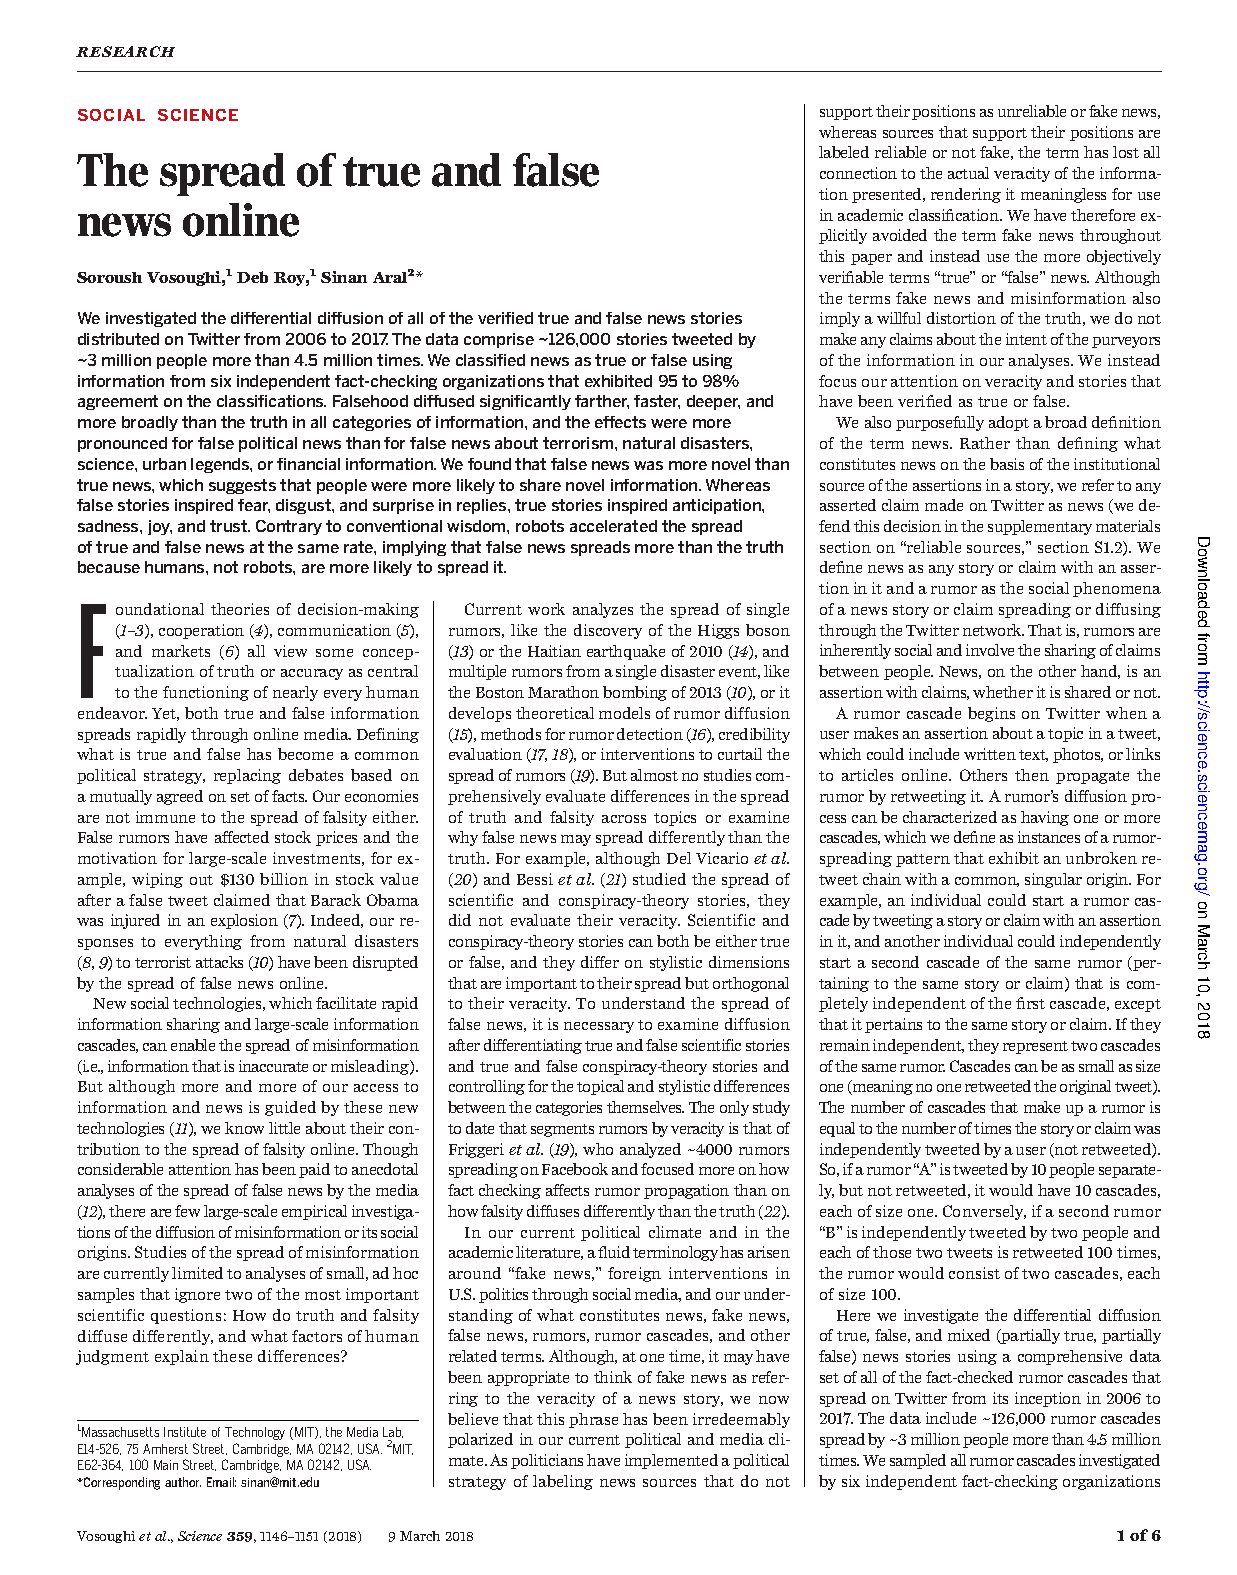
\includepdf[pages=1, scale=0.95, pagecommand=\heiti\sanhao{外\quad{}文\quad{}原\quad{}文}]{docs/translation.pdf}
\includepdf[pages=2-, scale=0.95, pagecommand={}]{docs/translation.pdf}
\end{center}

\end{document}